\chapter{词典}
dictionary 和 map 的区别是dict运行多个词条拥有相同的关键码,而map则不允许拥有相同的关键码

\section{skip list 跳转表}
\subsection{四联表 quadlist}
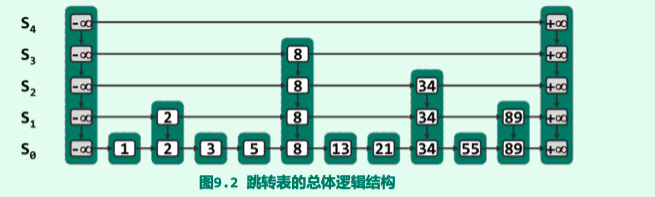
\includegraphics[scale=0.5]{5-42}\\
\begin{itemize}
\item 纵向的生长,依据生长概率逐层减半的原则
\item 第$k$层列表所含节点的期望数目: $\mathrm{E}\left(\left|\mathrm{S}_{k}\right|\right)=\mathrm{n} \times 2^{-\mathrm{k}}$
\item 空间总体消耗量的期望值: $E\left(\Sigma_{k}\left|S_{k}\right|\right)=\Sigma_{k} E\left(\left|S_{k}\right|\right)=n \times\left(\Sigma_{k} 2^{-k}\right)<2 n=O(n)$
\item 时间复杂度: 
\end{itemize}

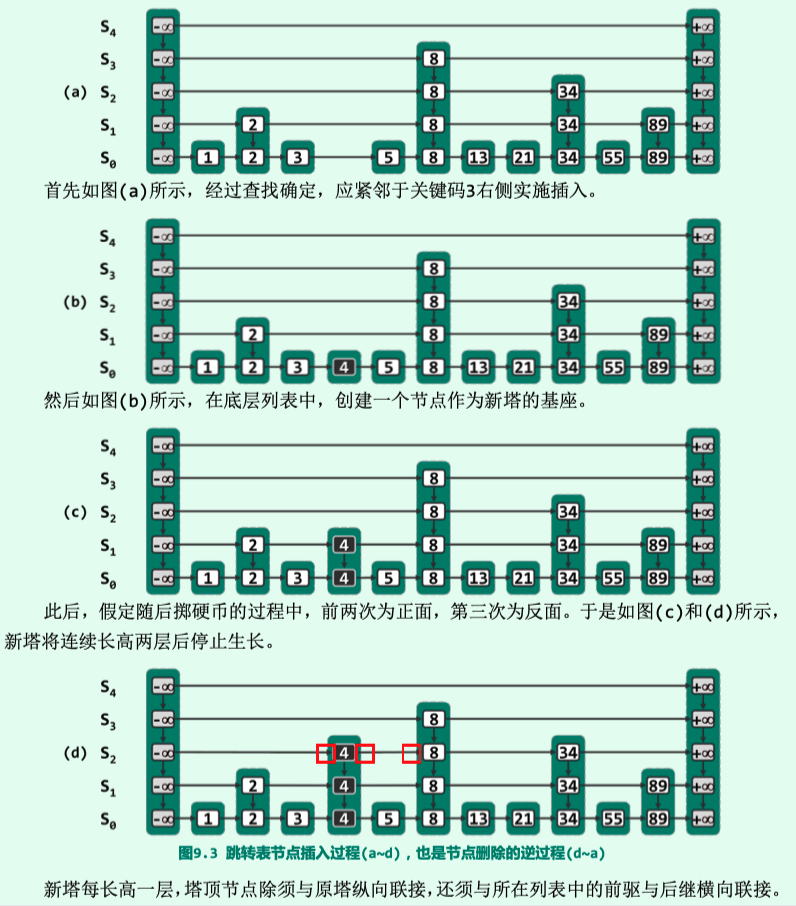
\includegraphics[scale=0.5]{5-43}

\section{散列表 hashtable}

\begin{itemize}
\item 可存放词条或引用的单元组成(bucket),线性结构,通常由向量来实现
\item bucket array
\item hash function: 词条与桶地址之间约定某种映射关系,hash(): key $\rightarrow$ hash(key): hashing address
\end{itemize}

\subsection{hash function}
\paragraph{division method}
mod,除数必须是素数,降低冲突的风险

\paragraph{MAD multiply-add-divide method}
(a $\times$ key + b) mod M, a > 0, b > 0, M为素数

\begin{itemize}
\item 数字分析法
\item 平方取中法
\item folding
\item xor
\item 分割后各区段的方向往复折返式
\item 伪随机数发
\item ...
\end{itemize}

\subsection{冲突及其排解}
\paragraph{multiple slots}
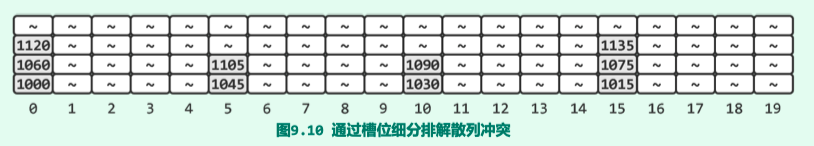
\includegraphics[scale=0.5]{5-44}
\begin{itemize}
\item 大部分slots都处于空闲状态,k个槽位的散列表可以讲装填因子降至之前的$\frac{1}{k}$
\end{itemize}

\paragraph{separate chaining}
\includegraphics[scale=0.5]{45}
\begin{itemize}
\item 子字典通过词典实现,而不是采用列表(向量)
\item 有效降低空间消耗,查找过程中发生冲突,需要遍历整个列表,导致查找成本的增加
\end{itemize}

\paragraph{公共溢出区 overflow area}
\begin{itemize}
\item 一旦插入词条发生冲突就转入公共缓冲池
\item 独立链等策略便捷而紧凑,但绝非上策。比如,因需要引入次 结构,实现相关算法的代码自身的复杂程度和出错概率都将加大大增加。反过来,因不能保证物 理上的关联性,对于稍大规模的词条集,查找过程中将需做更多的I/O操作。
\end{itemize}


\paragraph{闭散列策略}
只允许在散列表内部为其寻找另一空桶,closed hashing。之前在列表外开辟空间,称为open hashing

\begin{itemize}
\item linear probing: 若 hash(key) 被占用,转而试探hash(key)之后的捅,直至找到空桶为止
\begin{itemize}
\item 装填因子: $\lambda=N / M < 0.5$
\item 查找链: 从重复的位置开始
\item 局部性: 当散列表规模不小,装填因子不大的时候,闭散列对I/O负担的降低是更好的选择
\item 懒惰删除: 当词条直接删除,会导致后续所有查找的失败,如果需要删除对象,直接将桶的标志位ht[r]表姐为lazilyRemoved(t)
\item 删除查找: 当桶为空且没有remove标志才算``查找失败''
\item 插入查找: 当桶为空或带有remove标志,则可以用于插入
\item 重散列: 当装填因子越过某一个阈值时,调用rehash()算法
\end{itemize}
\end{itemize}

\paragraph{更多闭散列策略}
\begin{itemize}
\item linear probing 会加剧聚集现象
\item quadratic probing: 缓解聚集现象
\begin{itemize}
\item 确保试探终止: linear probing试探一遍必然停止;quadratic probing 要保证 $\lambda \leq 50\%$才能保证试探终止于某个空桶
\end{itemize}
\item pseudo-random probing
\item double hashing: 发现ht[hash(key)]被占用之后,以hash$_2$(key)为偏移量进行尝试: [hash(key) + i $\times$ hash2 (key)] \% M
\end{itemize}

\paragraph{散列码转换}
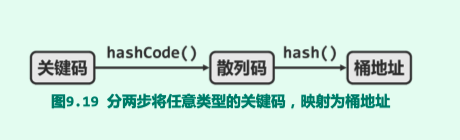
\includegraphics[scale=0.5]{5-46}
\begin{itemize}
\item 不超过32位的转成32位
\item 超过32位的分成高低32位求和
\item 字符串采用多项式散列码(polynomial hash code)
\end{itemize}

\section{散列应用}
\subsection{桶排序 bucketsort}
\begin{itemize}
\item 非重复情况直接使用关键码对应秩置位
\item 重复情况,使用独立链表,重复的置于链表之中
\end{itemize}

\subsection{基数排序 radixsort}
\begin{itemize}
\item least significant digit first: 低位字段优先
\item 时间复杂度: $O(t*(n+M))$
\end{itemize}

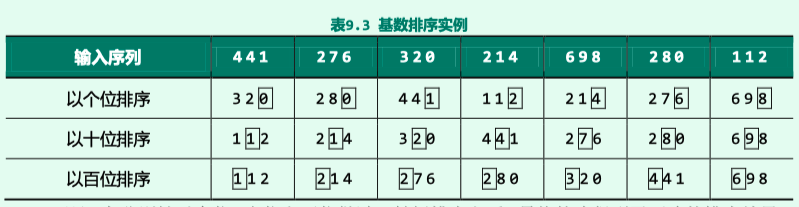
\includegraphics[scale=0.5]{5-47}

\chapter{优先级队列}
\begin{itemize}
\item 搜索树: 显式全序结构(full-order)
\item 散列表: 隐式全序结构(full-order),类似牺牲空间加快搜索速度
\item dictionary: 只要求关键码可以判等
\item priority queue: 要求关键码可以比较大小
\end{itemize}

\section{priority}
\subsection{huffman 编码树}
列表和向量对于优先级的理解过于机械,始终都保存了全体词条之间的全序关系,难以提高效率

\section{堆 heap}
\subsection{完全二叉堆}

\paragraph{插入--- 上滤}
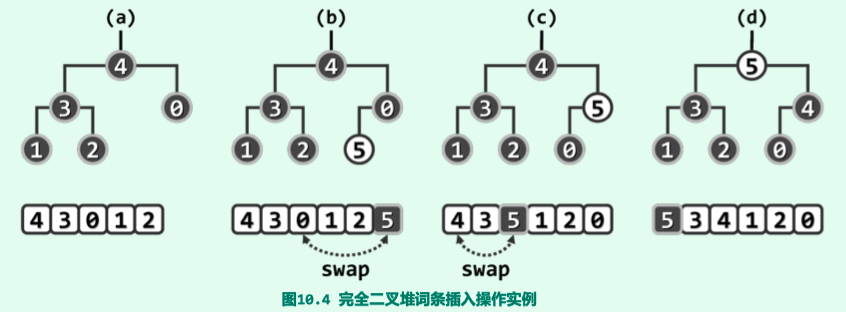
\includegraphics[scale=0.5]{5-48}

\paragraph{删除--- 下滤}
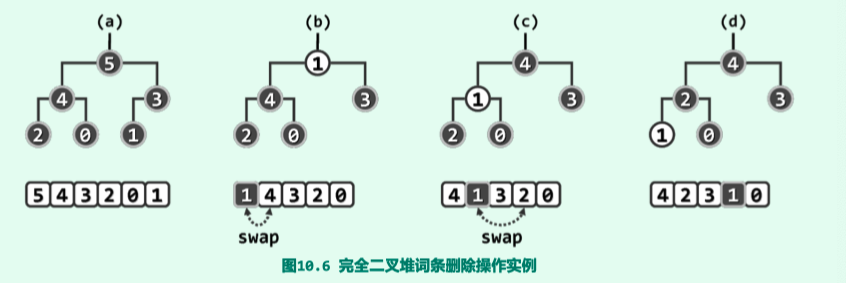
\includegraphics[scale=0.5]{5-49}

\paragraph{建堆 heapification}
\begin{itemize}
\item 蛮力算法: 时间复杂度$O({nlogn})$
\item Floyd算法: 堆合并操作, 自下而上的下滤, 时间复杂度$O({n})$\\
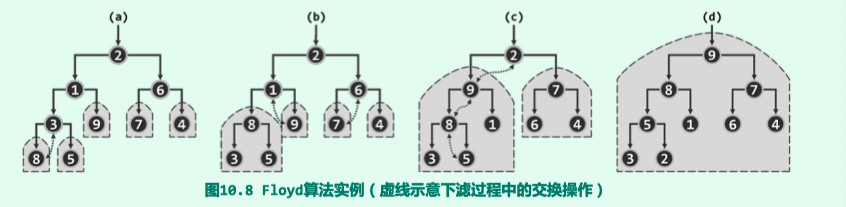
\includegraphics[scale=0.5]{5-50}
\end{itemize}

\subsection{就地堆排序 in-place heapsort}
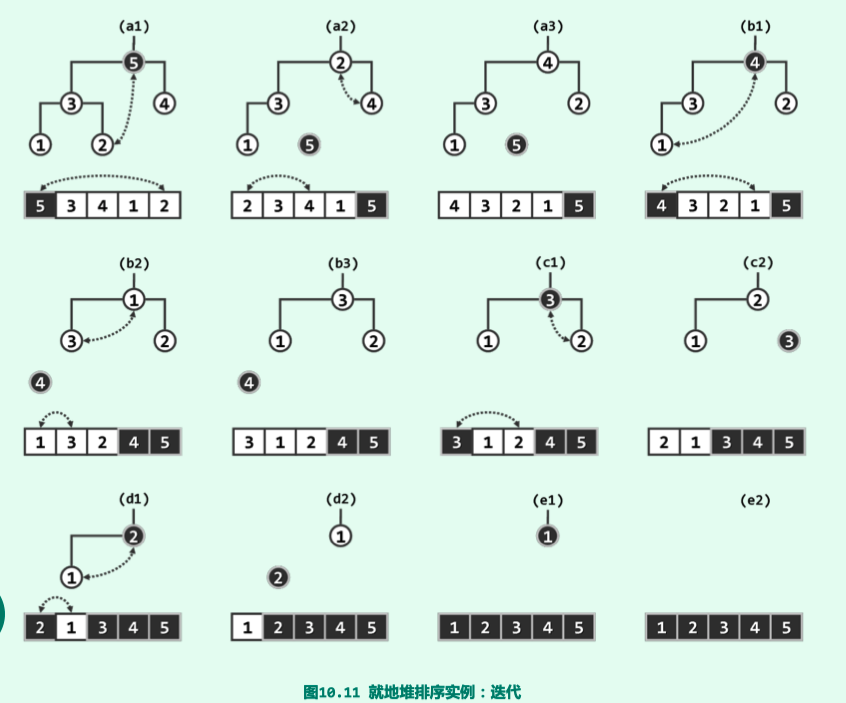
\includegraphics[scale=0.5]{5-51}

\section{左式堆}
两个堆进行合并组成一个堆

\subsection{单侧倾斜}
\paragraph{leftist heap}
左倾性: 任一内部节点x都满足左孩子不小于其右孩子,但前者的高度可能小于后者的高度\\
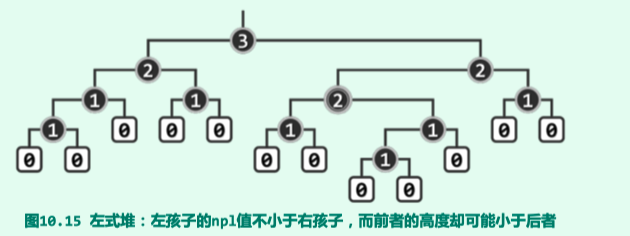
\includegraphics[scale=0.5]{5-52}

\paragraph{最右侧通路 rightmost path}
根节点的最右侧通路是全堆中深度最小的外部节点

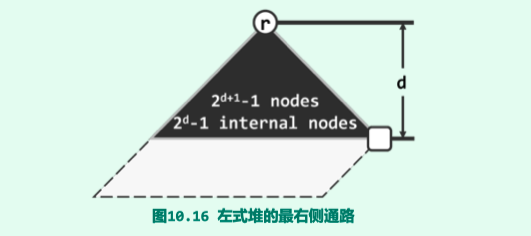
\includegraphics[scale=0.5]{5-53}

\paragraph{合并算法}
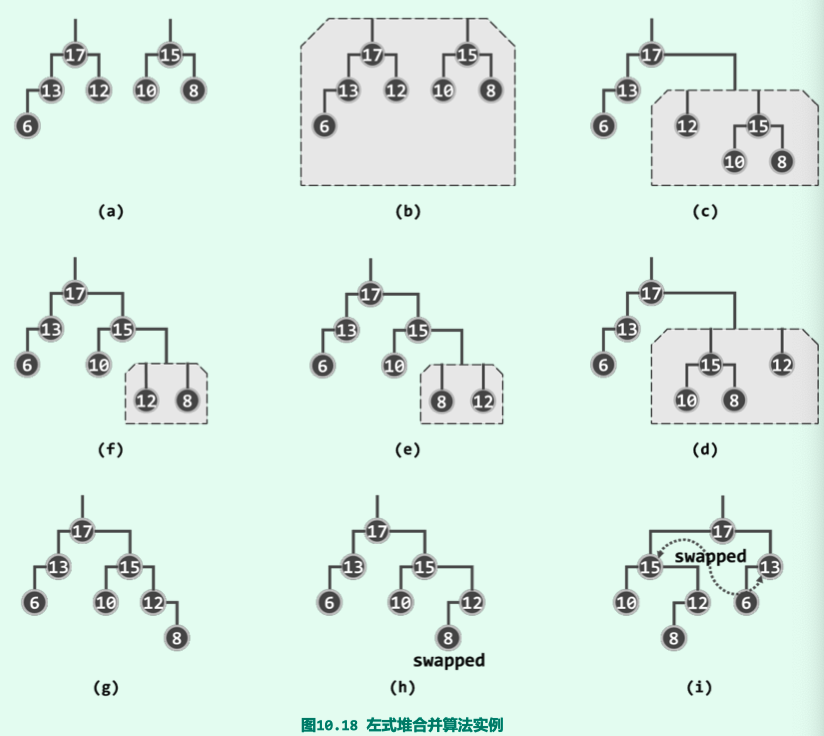
\includegraphics[scale=0.5]{5-54}

\chapter{串}
\begin{itemize}
\item call-by-pattern
\item 模式检测 (pattern detection)
\item 模式定位 (pattern location)
\item 模式计数 (pattern counting)
\item 模式枚举 (pattern enumeration)
\end{itemize}

\section{蛮力算法}
\begin{itemize}
\item 需要n-m+1次比对,每次比对需要比对至多m次,总体最差情况消耗时间$O(n*m)$
\end{itemize}

\section{KMP算法}
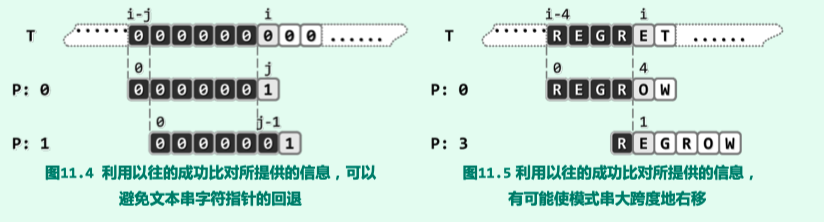
\includegraphics[scale=0.5]{5-55}
\begin{itemize}
\item 11.4中可以看出,利用KMP不需要回退i,而是保持i不变,根据P的特性,j只需要回退到j-1即可
\item 11.5可以看出,不需要回退i,而是将j回退到1
\item 这种方法利用了匹配的substring找到proper prefix和proper suffix重叠的长度t,使得j = j-t, i 保持不变\\
$next[j] = \max(N(P, j))=\max\{\theta \leq t<j \mid P[\theta, t)=P[j-t, j)\}$
\item 这个next表格可以由pattern p提前计算得出
\end{itemize}

\subsection{KMP改进}
由于$T[i] \neq p[j]$ 导致的错配,那么p[t]=p[j]时,对应的字符只会匹配失败,所以判定条件改为$\mathrm{N}(\mathrm{P}, \mathrm{j})=\{\theta \leq \mathrm{t}<j \mid \mathrm{P}[\theta, t)=P[j-t, j)$ 且 $P[t] \neq P[j]\}$

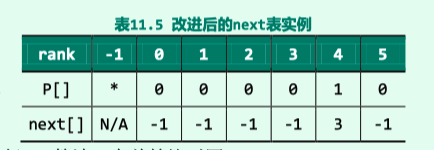
\includegraphics[scale=0.5]{5-56}

\section{BM算法}
采用自右向左匹配的方式\\
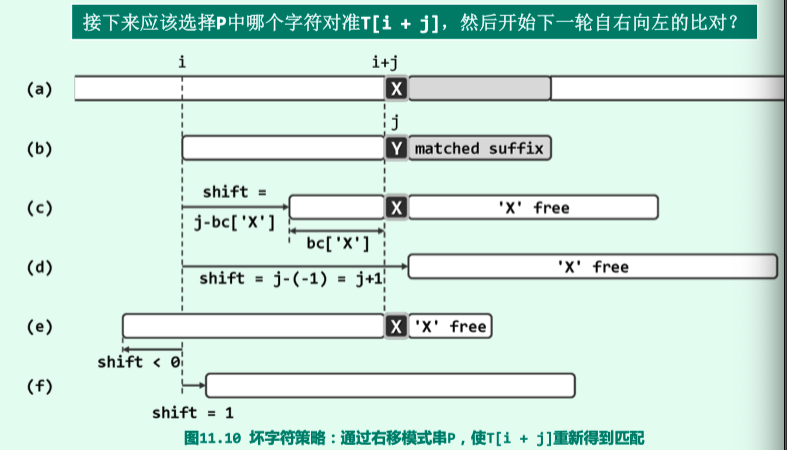
\includegraphics[scale=0.5]{5-57}

其中T[i+j]对应的是错配的字符,在后续的未匹配字符中如果没有T[i+j],那么字符串可以直接移动全长,否则移动到T[i+j]出现的位置再次匹配

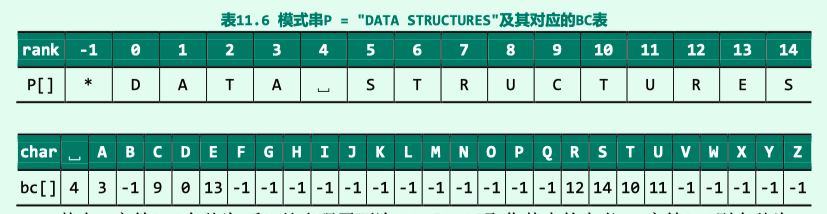
\includegraphics[scale=0.5]{5-58}

bc表的制作方法,char只存储最右侧的x对应的序号,与比对的方向相一致,最坏情况$O(n*m)$

\paragraph{改进}
不论T[i+j]与未匹配的前缀的匹配结果,最终还是要已匹配的后缀和未匹配的前缀相结合,所以应该对照pattern制作一个表格表明在该匹配位置出错之后pattern应该如何向右移动。最差运行时间O(n+m)\\
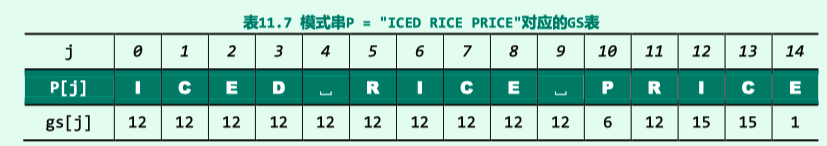
\includegraphics[scale=0.5]{5-59}

\paragraph{gs[]表构造原则}
ss[]标识真后缀的长度

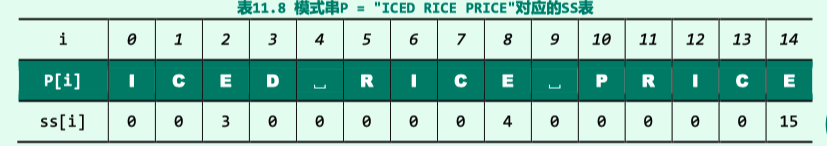
\includegraphics[scale=0.5]{5-60}

\section{karp-rabin算法}




















